\section{Terminal Model, Assumptions and Problem}
\subsection{Plant, controller and sampling convention}
The reused source terminal \cite{source} has two axes with angle $q\in\mathbb R^2$, angular rate $v$, delivered torque $a$ and PID integral $I$. Its nominal unsaturated equations are
\begin{align}
\dot q&=v,&J_a\dot v&=a-dv,\nonumber\\
\tau_a\dot a&=u_c-a,&\dot I&=q_m-r,\label{eq:plant}
\end{align}
\begin{align}
u_{\rm raw}&=-J_0k_p(q_m-r)+(d-J_0k_d)v_m-J_0k_iI,\nonumber\\
u_c&=\operatorname{clip}_{u_{\max}}(u_{\rm raw}).\label{eq:pid}
\end{align}
Clips act componentwise on torque and rate. At a rate boundary, outward acceleration is set to zero; the angle derivative uses clipped rate. Anti-windup freezes the integral derivative when the raw torque exceeds the torque limit. The model is advanced by held-disturbance RK4 with $h=0.02$~s. Each stored state is the state before that step; sensing occurs before the new reference is chosen, and the held reference and resulting torque apply to the following integration interval. Replay uses this convention, including the final next state.

The nominal controller uses $J_0$ even when the actual actuator differs. The declared actual model set is exactly
\begin{equation}
\mathcal M=\{.8,1,1.25\}\times\{1,1.5\},\quad
(J_a,\tau_a)=(J_0m_1,\tau_0m_2).
\label{eq:models}
\end{equation}
It contains six points. Membership between these points is not certified by interpolation or endpoint testing.

\subsection{Optical power and measured channels}
For boresight offset $b$, divergence $\alpha$ and positive scalar gain $g$,
\begin{align}
p&=p_0(\alpha)g\exp[-2\norm{q+b}^2/\alpha^2],\label{eq:powerplant}\\
p_0(\alpha)&=P_t\eta_o\left[1-\exp\left(-\frac{2r_a^2}{L^2\alpha^2}\right)\right].\nonumber
\end{align}
Service is available at a sampled instant when $p\geq p_{\min}$. Here $L$ is range and $r_a$ aperture radius. Receiver-side pointing, orbital propagation, atmospheric losses, queues and routing are outside this single-terminal experiment.

The measurements have separate physical noise scales:
\begin{align}
q_m&=q+\sigma_q Z_q,&[\sigma_q]&=\mathrm{rad},\nonumber\\
v_m&=v+\sigma_v Z_v,&[\sigma_v]&=\mathrm{rad/s},\label{eq:sensors}\\
p_m&=\max\{0,p(1+\sigma_p Z_p)\},&[\sigma_p]&=1.\nonumber
\end{align}
There are five scalar channels: two angles, two rates and one relative-power disturbance. The inherited kernel uses numeric noise coefficient $\sigma_q$ for the encoder and twice that numeric value for the rate. We document this source policy dimensionally as $\sigma_v=\gamma_v\sigma_q$, $\gamma_v=2~\mathrm{s}^{-1}$. This resolves the written unit mismatch without changing any inherited sensor value. It is not an independently calibrated hardware relationship. Direct source-kernel checks reproduce 2,100 sensor samples at three noise scales with zero numerical discrepancy; the new traces retain explicit rate-unit metadata.

\begin{table}[t]
\caption{Terminal values and provenance. All physical values are assumptions; source-derived values describe implementation rather than independent calibration.}
\centering\footnotesize\setlength{\tabcolsep}{4pt}
\begin{tabular}{@{}p{.36\columnwidth}p{.40\columnwidth}p{.17\columnwidth}@{}}\toprule
Quantity & Value & Provenance\\\midrule
Range / aperture diameter & 800 km / 0.10 m & Assumed\\
$P_t,\eta_o,\alpha$ & 0.5 W, 0.4, $20\um$ & Assumed\\
$\alpha$ interval & $[18,22]\um$ & Assumed\\
Aligned $p_0$, $p_{\min}$ & 3.9062, 1.5 $\mu$W & Derived / assumed\\
$J_0,d,\tau_0$ & .002 kg m$^2$, .004 N m s/rad, .08 s & Assumed\\
$k_p,k_d,k_i$ & 64 s$^{-2}$, 14 s$^{-1}$, 8 s$^{-3}$ & Source-derived\\
Torque / rate limit & $2~\mu$N m / $120\um$/s & Assumed\\
Base $\sigma_q,\sigma_v$ & $.08\um$, $.16\um$/s & Source policy\\
Base $\sigma_p$, coupling $\gamma_v$ & .008, 2 s$^{-1}$ & Source policy\\
Sample / mission & .02 s / 14 s ($N=700$) & Protocol\\
Prior $\norm b$, maximum gain & $30\um$, 1.05 & Assumed\\
Working / acquisition budget & 0 s / 4 s & Protocol\\\bottomrule
\end{tabular}
\label{tab:model}
\end{table}

\subsection{Numbered assumption contract}
The theorem below uses the following hypotheses.
\begin{enumerate}
\item[A1.] The starting power is positive; $b$ and $\alpha$ remain constant during the candidate window; $\alpha\in[\alpha_-,\alpha_+]$ and $\norm b\leq b_{\max}$.
\item[A2.] $0<g(t_0)\leq g_{\max}$ and $\log[g(t_0+s)/g(t_0)]\geq-\ell s$ at all evaluated samples, for declared $\ell\geq0$.
\item[A3.] Actual $(J_a,\tau_a)$ belongs to \eqref{eq:models}; the source sampled dynamics and nominal controller apply. The initial state is zero, pre-probe reference is zero, and there is at most one attempt per mission.
\item[A4.] Encoder and rate bias are zero. All five standardized sensor disturbances have the declared marginal Gaussian tails and correct scales over all $N$ mission samples. Cross-channel or temporal independence is not needed for the union bound.
\item[A5.] Candidate RK4-stage torque and rate enclosures lie strictly within their clamps. Candidate duration fits the declared horizon. Optical and sensor evidence is valid for the requested window.
\end{enumerate}
A simulation record can check injected histories against this contract, but cannot establish the physical truth of A1--A5 for a real terminal. Evidence references are required by the supervisory interface; mere reference presence does not authenticate calibration or future fault constancy.

\begin{table}[t]
\caption{Recurring notation and dimensions.}
\centering\footnotesize
\begin{tabular}{@{}p{.25\columnwidth}p{.68\columnwidth}@{}}\toprule
Symbol & Meaning / dimension\\\midrule
$h,N,\delta$ & Sample time (s), mission samples, failure allowance\\
$e_0,d_i$ & Starting angular error, delivered increment (rad)\\
$c,R,\bar d_i,r_i$ & Centers and radii of error/increment balls (rad)\\
$\overline D_i$ & Upper change in squared angular loss (rad$^2$)\\
$\ell,\kappa,\eta$ & Log-gain decline (s$^{-1}$), tail quantile, relative envelope\\
$\underline p_i,B$ & Power lower bound (W), sampled outage budget (s)\\
$M,H,K$ & Number of models, window samples, candidates\\
$\rho_x,F,C_b$ & State box radii, projected information, offset covariance\\\bottomrule
\end{tabular}
\end{table}

\subsection{Authorization objective and four separate properties}
Given a candidate reference, measured start and its proposed displacement enclosure, compute $\underline p_i$ such that actual sampled window outage obeys
\begin{equation}
h\sum_{i=0}^{H-1}\mathbf1\{p_i<p_{\min}\}
\leq h\sum_{i=0}^{H-1}\mathbf1\{\underline p_i<p_{\min}\}\leq B
\label{eq:objective}
\end{equation}
under the contract. This authorizes sampled service for that probe only. It does not bound the offset estimation error, guarantee a correct diagnosis, or authorize a post-probe correction. The estimator and recovery logic in Fig.~\ref{fig:flow} remain separate from the blue permission path.

\begin{figure*}[t]
\centering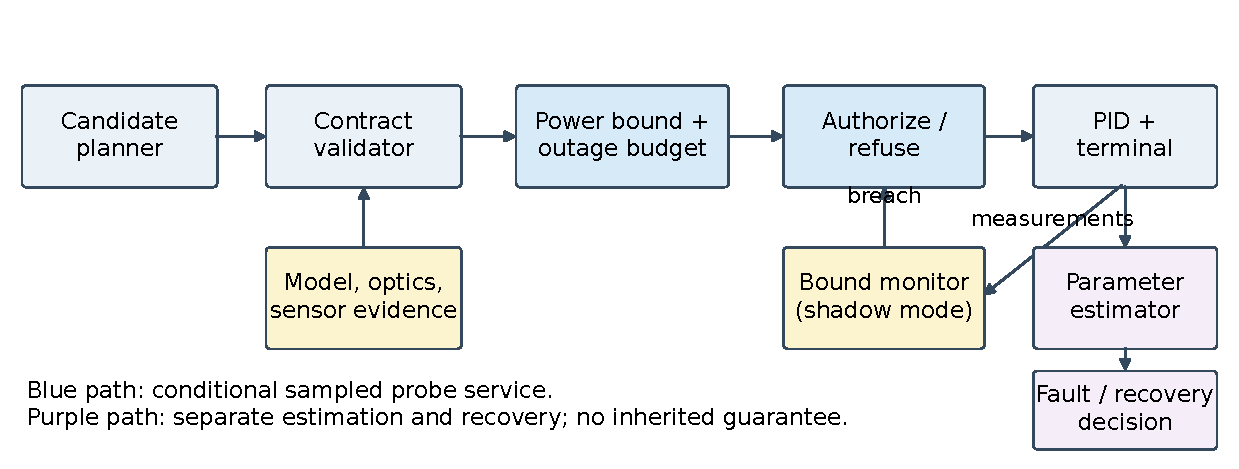
\includegraphics[width=\textwidth]{information_flow.pdf}
\caption{Information flow and guarantee boundary. Evidence validation precedes conditional permission. Estimation and recovery consume measurements but do not inherit the probe-window service theorem. The supplied implementation is a simulation/shadow interface.}
\label{fig:flow}
\end{figure*}
